\chapter{Lecture 8: Consequences of Cauchy's Integral Formula}

\begin{theorem}
    if $f(z)$ is analytic in a domain $D, z_0 \in D$ and $\{|z-z_0| < R\} \subseteq D$, then $f(z)$ hasa convergent power series expansion about $z_0$ given by:
    \begin{equation}
        f(z) = \sum_{n=0}^{\infty} a_n(z-z_0)^n
    \end{equation}
    Where:
    \begin{equation}
        a_n = \frac{1}{2\pi i} \int_{\gamma} \frac{f(z)}{(z-z_0)^{n+1}} dz
    \end{equation}
    for any simple, closed, positively oriented curve $\gamma$ in $D$ containing $z_0$ and $\gamma=|z-z_0| = R$.
\end{theorem}

\begin{proof}
    Let $\Delta = \{|z-z_0| < R\}$. if $z \in \Delta$, $|z - z_0| = s < R$, then by Cauchy's Integral Formula:
    \begin{equation}
        f(z) = \frac{1}{2\pi i} \int_{\gamma} \frac{f(\zeta)}{\zeta - z} d\zeta
    \end{equation}
    Where $\gamma = \{|z - z_0| = r\}$, positively oriented, $r > s$.\\
    \begin{figure}[H]
        \centering
        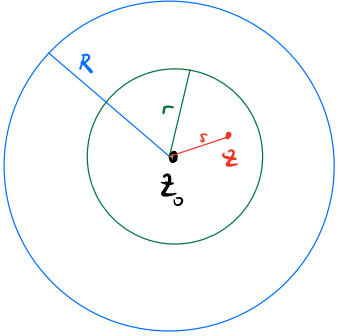
\includegraphics[scale=0.5]{LECTURE_8/proof.png}
    \end{figure}
    Now we write:
    \begin{align*}
        \xi - z & = \xi -z_0 - (z - z_0)                                   \\
                & = (\xi - z_0) \left(1 - \frac{z - z_0}{\xi - z_0}\right) \\
    \end{align*}
    Since $\frac{z - z_0}{\xi - z_0}  = \frac{s}{r} < 1$, we can write (for $\xi \in \gamma$):
    \begin{equation}
        \frac{1}{1 - \frac{z - z_0}{\xi - z_0}} = \sum_{k=0}^{\infty} \left(\frac{z - z_0}{\xi - z_0}\right)^k \qquad \text{Geometric Series}
    \end{equation}
    So, \textit{for any $N \in \mathbb{N}$ we have}:
    \begin{align*}
        f(z) & = \frac{1}{2\pi i} \int_{\gamma} \frac{f(\xi)}{\xi - z_0} \sum_{k=0}^{\infty} \left(\frac{z - z_0}{\xi - z_0}\right)^k d\xi                  \\
             & = \sum_{k=0}^{N} (z - z_0)^k \left(\frac{1}{2\pi i} \int_{\gamma} \frac{f(\xi)}{(\xi - z_0)^{k+1}} d\xi\right)                               \\
             & + \frac{1}{2\pi i} \int_{\gamma} \frac{f(\xi)}{\xi - z_0} \left[ \sum_{k=N+1}^{\infty} \left(\frac{z - z_0}{\xi - z_0}\right)^k \right] d\xi
    \end{align*}
    Since $\sum_{k=0}^{\infty} \frac{|z - z_0|^k}{|\xi - z_0|^k}$ converges, if $\epsilon > 0$\\
    We can choose $L$ such that $\forall N > L$ we have:
    \begin{equation}
        \sum_{k=N+1}^{\infty} \frac{|z - z_0|^k}{|\xi - z_0|^k} < \epsilon
    \end{equation}
    Since $f$ analytic, there is a constant $M$ such that $\max|f(\xi)| \leq M$ for $\xi \in \gamma$.\\
    By definition: $|\xi - z_0| = r$ on $\gamma$, thus, by the triangle inequality:
    \begin{align*}
        \frac{1}{2\pi i} \int_{\gamma} \frac{f(\xi)}{\xi - z_0} \left[ \sum_{k=N+1}^{\infty} \left(\frac{z - z_0}{\xi - z_0}\right)^k \right] d\xi \geq \frac{\text{length}(\gamma)}{r} M \epsilon = 2\pi M \epsilon
    \end{align*}
    Thus, $\forall \epsilon > 0, \exists L | \forall N > L$ we have:
    \begin{equation}
        \left| f(z) - \sum_{k=0}^{N} a_k(z - z_0)^k \right| < 2\pi \epsilon
    \end{equation}
    Where $a_k = \frac{1}{2\pi i} \int_{\gamma} \frac{f(\xi)}{(\xi - z_0)^{k+1}} d\xi$.
    So: $f(z) = \sum_{k=0}^{\infty} a_k(z - z_0)^k$. as desired.

\end{proof}
\begin{corollary}
    If $f(z)$ is analytic in a domain $D$, then so is $f'(z)$. In particular, if $f$ is analytic, then it is infinitely differentiable.
\end{corollary}

\begin{proof}
    Every $f$ has a power series expansion about $z_0$, and every term in the series is analytic. Therefore, the series converges to an analytic function.
\end{proof}

\begin{corollary}
    [Unique Analytic Continuation] If $f(z)$ is analytic in a domain $D$, and $f(z) = 0$ for all $z \in \Delta \subseteq D$, then $f(z) = 0$ for all $z \in D$.
    In the above setting we have:
    \begin{equation}
        \frac{f^{(k)}(z_0)}{k!} = \frac{1}{2\pi i} \int_{\gamma} \frac{f(\xi)}{(\xi - z_0)^{k+1}} d\xi
    \end{equation}
    In particular, if $f$ is analytic in a domain $D$, and, for some $z_0 \in D$, $f^{(k)}(z_0) = 0$ for all $k \in \mathbb{N}$, then $f(z) = 0 \forall z \in D$.
\end{corollary}
\section{Comparison with Real Functions}

\begin{example}
    To get a sense for the difference between real and complex functions, consider the following \textbf{real function}:
    \begin{equation}
        f(x) = \begin{cases}
            e^{-1/x^2} & x > 0    \\
            0          & x \leq 0
        \end{cases}
    \end{equation}
    $f$ is infinitely differentiable, and $\forall k \in \mathbb{N}$, $f^{(k)}(0) = 0$.\\
    So, the Taylor series of $f$ at $0 \in \mathbb{R}$ is:
    \begin{equation}
        f(x) = \sum_{k=0}^{\infty} \frac{f^{(k)}(0)}{k!} x^k = 0
    \end{equation}
    Thus, $f$ is infinitely differentiable, but \textbf{\underline{\textit{not}}} equal to a power series in any neighborhood of $0\in \mathbb{R}$.
\end{example}